\documentclass{beamer}
\usetheme{Boadilla}
\usepackage[T1]{fontenc}

\title{Redundantny system plików}

\author{Kacper Pieniążek}
\date{\today}

\begin{document}
	\begin{frame}
		\titlepage
	\end{frame}

	\section{Section 1}
	\subsection{sub a}
	
	\begin{frame}
		\frametitle{Cel pracy}
			System plików zapewniający ochronę danych nawet w przypadku ich uszkodzenia w oparciu o interfejs FUSE.
	\end{frame}
	
	\begin{frame}
		\frametitle{Technologia}
            \begin{block}{Filesystem in Userspace}
			    Moduł jądra systemów Linuxowych umożliwiający tworzenie systemu plików w przestrzeni użytkownika. Moduł FUSE stanowi połączenie między jądrem, a implementowanym systemem.
            \end{block}
	\end{frame}


	\begin{frame}
		\frametitle{Założenia pracy}
		\begin{itemize}
			\item Wykrywanie niezgodności danych
				\begin{itemize}
					\item Sumy kontrolne
					\item Kody korekcyjne
				\end{itemize}
			\pause
			\item Odzyskiwanie danych
			\begin{itemize}
				\item Duplikacja danych
				\item Kody korekcyjne
			\end{itemize}
			\pause
			\item Podstawowa funkcjonalność systemu plików
			\begin{itemize}
				\item Odczyt, zapis, tworzenie, usuwanie plików
                \item Tworzenie oraz usuwanie katalogów
			\end{itemize}
			\pause
			\item Wygodne użytkowanie
			\begin{itemize}
				\item Podział i duplikacja danych wystarczająco transparentna dla użytkownika
				\item Rozwiązywanie konfliktów w przypadku niezgodności danych
				\item Dostosowanie systemu do własnych potrzeb
			\end{itemize}
		\end{itemize}
	\end{frame}
	
	\begin{frame}
		\frametitle{Analiza problemu}

		\begin{itemize}
			\item Jak zapewnić redundancję?
			\pause 
		    \item Jak wykrywać rozbieżność danych?
			    \begin{itemize}
				    \item Podczas operowania na uszkodzonych danych; błędny odczyt, kody korekcyjne, sumy kontrolne 
			    \end{itemize}
            \item Jak zapewnić spójność danych?
			\pause
            \begin{itemize}
				\item Synchronizacja między replikami, wybór poprawnych danych
			\end{itemize}
		    \pause
			\item Jak naprawiać rozbieżność danych?
			
		\end{itemize}
	\end{frame}
		
	\begin{frame}
		\frametitle{Rozwiązanie}
			\begin{block}{Definicja}
				Replika - Katalog zawierający kopię chronionych danych
			\end{block}
			\begin{itemize}
				\item System replik oparty na rozwiązaniach architektury RAID
				\begin{itemize}
					\item Podział danych w replikach oparty na poziomach RAID-0, RAID-1
				\end{itemize}
			\end{itemize}
			
	\end{frame}

		
\begin{frame}
	\frametitle{Rozwiązanie}
	\begin{block}{Definicja}
	    Replika standardowa - detekcja błędów w plikach, jednak w przypadku wykrycia takiego błędu, nie jest w stanie dokonać samodzielnej korekty
    \end{block}
	\begin{block}{Definicja}
        Replika korekcyjna - dokonuje zarówno detekcji, jak i korekcji znalezionych błędów
    \end{block}
    Jeśli naprawa błędów w replice jest niemożliwa, uszkodzone dane są zastępowane kopiami z pozostałych replik.
\end{frame}

\begin{frame}
        \frametitle{Replika blokowa}
		\begin{columns}
		\column{0.7\textwidth}
		\begin{block}{Redundancja}
			Standardowa replika blokowa rozkłada pliki na kilka mniejszych części, do każdego dołączając informacje potrzebne do detekcji błędów
		\end{block}
		\begin{itemize}
			\item Podstawa repliki korekcyjnej 
			\item Dwa podziały:
			\begin{itemize}
				\item Bloki stałej długości
				\item Bloki zmiennej długości
			\end{itemize}
			\item Operacje read, write, open, close, stat
			\item Podział danych niewidoczny dla użytkownika
			\item Podział na bloki umożliwia naprawę tylko uszkodzonych części danych
		\end{itemize}
		\column{0.3\textwidth}
		\begin{figure}
			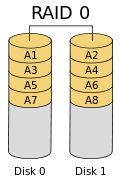
\includegraphics[scale=0.5]{raid-0.png}
		\end{figure}
		\end{columns}
\end{frame}

\begin{frame}
        \frametitle{Replika lustrzana}
	\begin{columns}
		\column{0.6\textwidth}
		\begin{block}{Redundancja}
                Standardowa replika lustrzana zapisuje pliki w całości, dołączając informacje potrzebne do detekcji błędów.
		\end{block}
		\begin{itemize}
			\item Podstawa repliki korekcyjnej
			\item W przypadku naprawy zmianie ulega cały plik
		\end{itemize}
        \column{0.4\textwidth}
		\begin{figure}
			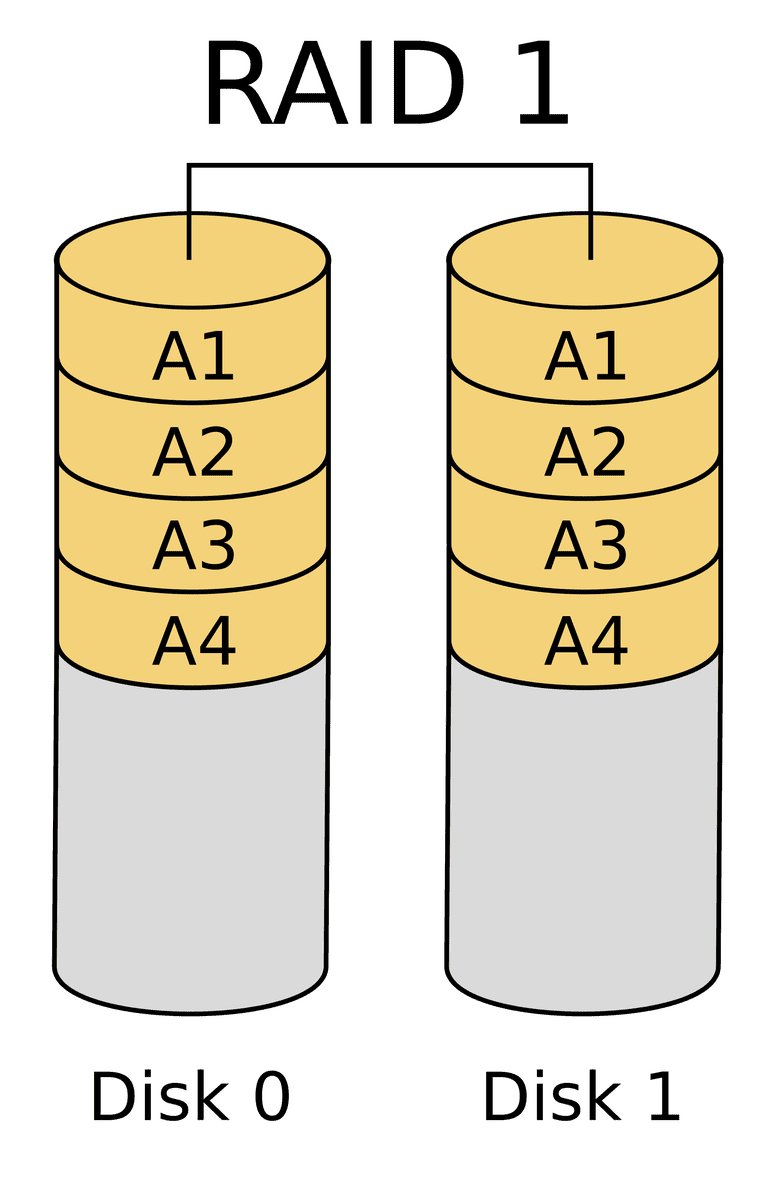
\includegraphics[scale=0.4]{raid-1.png}
		\end{figure}
	
	\end{columns}
\end{frame}
	
\begin{frame}
        \frametitle{Repliki korekcyjne }
	\begin{columns}
		\column{1.0\textwidth}
		\begin{block}{Korekcja błędóww}
		   Repliki korekcyjne są w stanie naprawiać własne błędy podczas operacji lub synchronizacji z innymi replikami.
        \end{block}
		\begin{itemize}
			\item Kod Hamminga 
			\item Bloki parzystości
		\end{itemize}

	\end{columns}
\end{frame}
			
	\begin{frame}
		\frametitle{Przykłady}
		\begin{block}{Przykład}
			Dysk, na którym znajdowała się jedna z replik, został odmontowany. 
		\end{block}
		\pause
		\begin{block}{Przykład}
			Wystąpił błąd podczas zapisu do jednej z replik blokowych.
		\end{block}
		\pause
		\begin{block}{Przykład}
			Odwrócone bity na danych w w replice.
		\end{block}
	\end{frame}
	

	\begin{frame}
		\frametitle{Ulepszenia}
		\begin{itemize}
			\item Wprowadzenie kolejnych rodzajów replik
            \item Wprowadzenie kolejnych metod detekcji i korekcji błędów
			\item Usprawnienie działania
			\begin{itemize}
				\item Wykorzystanie wywołań niskiego poziomu FUSE
				\item Optymalizacja obecnych rozwiązań 
			\end{itemize}
			\item Implementacja całej funkcjonalności systemu plików
                    \begin{itemize}
                        \item Obsługa pozostałych sygnałów biblioteki FUSE
                        \item Obsługa pozostałych typów plików
                    \end{itemize}
			\item Działanie systemu całkowicie niezależne od użytkownika
		\end{itemize}
	\end{frame}

\end{document}
